\section{Gaussian integral}

\textbf{Normal distribution}, a term often appeared in statistics, is defined
by equation (\ref{gauss-distr})

\begin{equation}
	p(x)={1\over\sigma\sqrt{2\pi}}
	e^{-\frac12\left(x-\mu\over\sigma\right)^2}
	\label{gauss-distr}
\end{equation}

in which $\sigma$ is the standard deviation (Accordingly, $\sigma^2$ is the
variance), and $\mu$ is the mean value. Since normal distribution is a
\textbf{probability density function}, it should always satisfies (\ref{pdf1})
and (\ref{pdf2}), where set $\mathbb{X}$ denotes all possible values of the
continuous variable $x$.

\begin{equation}
	\forall x\in\mathbb{X},p(x)\ge0
	\label{pdf1}
\end{equation}
\begin{equation}
	\int_{x\in\mathbb{X}} p(x)dx=1
	\label{pdf2}
\end{equation}

It is very easy to prove that $p(x)>0$ because the exponential function is
always positive for all real input. In this section, Condition in equation
(\ref{pdf2}) will be proven.

\subsection{Perform substitution to simplify the integral}

By simplifying the exponential function, we make the following substitutions.

$$
\begin{aligned}
	\frac12\left(x-\mu\over\sigma\right)^2=u^2 \\
	u={1\over\sqrt2}\left(x-\mu\over\sigma\right) \\
	du={dx\over\sigma\sqrt2} \\
	\therefore dx=\sigma\sqrt2du
\end{aligned}
$$

With the substitutions applied, the integral is transformed.

\begin{equation}
	{1\over\sigma\sqrt{2\pi}}\int_{-\infty}^\infty
	e^{-\frac12\left(x-\mu\over\sigma\right)^2}dx=
	{1\over\sigma\sqrt{2\pi}}\cdot\sigma\sqrt2\int_{-\infty}^\infty
	e^{-u^2}du
	={1\over\sqrt\pi}\int_{-\infty}^\infty e^{-u^2}du
	\label{gauss-distr-int}
\end{equation}

By proving $\int_{-\infty}^\infty e^{-u^2}du$, the Gaussian integral, is the
square root of $\pi$, we can then testify the normal distribution satisfies the
second identity of probability density functions.

\subsection{Find the square of the Gaussian integral}

Squaring the integral turns it into a double integral over the
cartesian plane of $(u,v)$, which is also visualized in figure \ref{gauss-3d}.

$$
\begin{aligned}
	\left(\int_{-\infty}^\infty e^{-u^2}du\right)^2
	&=\int_{-\infty}^\infty e^{-u^2}du\int_{-\infty}^\infty e^{-v^2}dv \\
	&=\int_{-\infty}^\infty\int_{-\infty}^\infty e^{-(u^2+v^2)}dudv
\end{aligned}
$$

\begin{figure}[ht]
	\centering{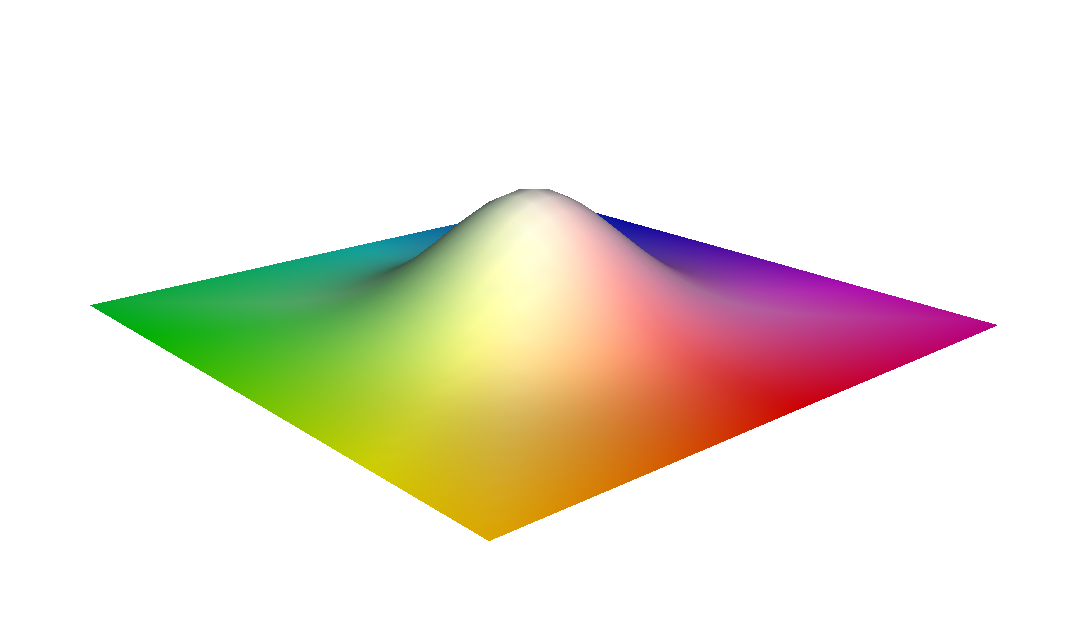
\includegraphics[width=4in]{graphics/gauss-3d.png}}
	\caption{Plot of function $z=e^{-(u^2+v^2)}$}\label{gauss-3d}
\end{figure}

\subsection{Simplify the integral by converting coordinate systems}

Ostensibly, the integral problem seems to become more complicated; however, it
becomes easier with the transformation from Cartesian coordinates to polar
coordinates via applying the rules in equation (\ref{car-to-pol}).

\begin{equation}
	\begin{cases}
		u=r\cos\theta \\
		v=r\sin\theta
	\end{cases}
	\label{car-to-pol}
\end{equation}

Since it is replacing two variables at the same time, the transformation itself
can be interpreted as a vector-valued function. Because $u$ and $v$ are
non-linearly transformed, a function will be needed to transform the tiny piece
$dudv$. Although it is a non-linear transform, a linear approximation for this
transform is made possible by \textbf{Jacobian matrix}.

$$
J=
\begin{bmatrix}
	{\partial u\over\partial r} & {\partial u\over\partial\theta} \\
	{\partial v\over\partial r} & {\partial v\over\partial\theta}
\end{bmatrix}
=
\begin{bmatrix}
	\cos\theta & -r\sin\theta \\
	\sin\theta & r\cos\theta
\end{bmatrix}
$$

Accordingly, $dxdy$ is approximated by the absolute value of the
\textbf{Jacobian determinant}.

$$
\left|\det(J)\right|=\left|r\cos^2\theta+r\sin^2\theta\right|=r
$$

As a result, the complicated double integral over Cartesian plane becomes an
easier double integral over polar regions.

$$
\int_{-\infty}^\infty\int_{-\infty}^\infty e^{-(u^2+v^2)}dudv
=\int_0^{2\pi}\int_0^\infty e^{-r^2}rdrd\theta
$$

\pagebreak
\subsection{Evaluate the double integral}

Since the inner function does not depend on the variable $\theta$, the outer
integral is treated separately.

$$
\int_0^{2\pi}\int_0^\infty e^{-r^2}rdrd\theta
=\int_0^{2\pi}d\theta\int_0^\infty e^{-r^2}rdr=2\pi\int_0^\infty e^{-r^2}rdr
$$

Now, let $a\triangleq-r^2$ so that the exponent is further simplified.

$$
\begin{aligned}
	\because a=-r^2 \\
	\therefore da=-2rdr \\
\end{aligned}
$$
$$
\begin{aligned}
	2\pi\int_0^\infty e^{-r^2}rdr
	&=\pi\int_{-\infty}^0 e^ada \\
	&=\pi\cdot\left.e^a\right|_{-\infty}^0=\pi\cdot1=\pi
\end{aligned}
$$

\subsection{Calculate Gaussian integral from the double integral}

Take the square root of the double integral yields the answer to the original
Gaussian integral.

$$\int_{-\infty}^\infty e^{-u^2}du=\sqrt\pi$$

Plugging the above result into equation (\ref{gauss-distr-int}) makes
(\ref{gauss-distr}) a genuine probability density function.

$$
{1\over\sqrt\pi}\int_{-\infty}^\infty e^{-u^2}du
={1\over\sqrt\pi}\cdot\sqrt\pi=1
$$
